\documentclass[11pt]{article}
\usepackage[utf8]{inputenc}
\usepackage{graphicx}
\usepackage{amsmath}
\usepackage{amssymb}
\usepackage{algorithm}
\usepackage{algpseudocode}
\usepackage{tikz}
\usetikzlibrary{shapes,arrows,positioning,calc}
\usepackage{hyperref}
\usepackage{geometry}
\usepackage{listings}
\usepackage{xcolor}

\geometry{a4paper, margin=1in}

% Define custom language styles for listings
\lstdefinelanguage{JavaScript}{
  keywords={typeof, new, true, false, catch, function, return, null, catch, switch, var, if, in, while, do, else, case, break},
  keywordstyle=\color{blue}\bfseries,
  ndkeywords={class, export, boolean, throw, implements, import, this},
  ndkeywordstyle=\color{darkgray}\bfseries,
  identifierstyle=\color{black},
  sensitive=false,
  comment=[l]{//},
  morecomment=[s]{/*}{*/},
  commentstyle=\color{purple}\ttfamily,
  stringstyle=\color{red}\ttfamily,
  morestring=[b]',
  morestring=[b]"
}

\lstdefinelanguage{JSON}{
    basicstyle=\normalfont\ttfamily,
    numbers=left,
    numberstyle=\scriptsize,
    stepnumber=1,
    numbersep=8pt,
    showstringspaces=false,
    breaklines=true,
    frame=lines,
    backgroundcolor=\color{gray!10},
    literate=
     *{0}{{{\color{blue}0}}}{1}
      {1}{{{\color{blue}1}}}{1}
      {2}{{{\color{blue}2}}}{1}
      {3}{{{\color{blue}3}}}{1}
      {4}{{{\color{blue}4}}}{1}
      {5}{{{\color{blue}5}}}{1}
      {6}{{{\color{blue}6}}}{1}
      {7}{{{\color{blue}7}}}{1}
      {8}{{{\color{blue}8}}}{1}
      {9}{{{\color{blue}9}}}{1}
      {:}{{{\color{red}{:}}}}{1}
      {,}{{{\color{red}{,}}}}{1}
      {\{}{{{\color{red}{\{}}}}{1}
      {\}}{{{\color{red}{\}}}}}{1}
      {[}{{{\color{red}{[}}}}{1}
      {]}{{{\color{red}{]}}}}{1},
}

\lstdefinelanguage{Python}{
    basicstyle=\normalfont\ttfamily,
    numbers=left,
    numberstyle=\scriptsize,
    stepnumber=1,
    numbersep=8pt,
    showstringspaces=false,
    breaklines=true,
    frame=lines,
    backgroundcolor=\color{gray!10},
    keywords={def, class, return, if, elif, else, for, while, import, from, as, try, except, finally, with, lambda, yield, assert, break, continue, del, global, not, and, or, in, is, None, True, False},
    keywordstyle=\color{blue}\bfseries,
    comment=[l]{\#},
    commentstyle=\color{green}\ttfamily,
    stringstyle=\color{red},
    morestring=[b]',
    morestring=[b]",
    emph={self},
    emphstyle=\color{magenta}\bfseries
}

\title{Adaptive Deep Bayesian Neural Network Framework: \\ Comprehensive Technical Documentation}
\author{Ninan sajeeth Philip\\ Artificial Intelligence Research and Intelligent Systems (airis4d.com)\\Thelliyoor 689544}
\date{\today}

\begin{document}

\maketitle

\begin{abstract}
This document provides comprehensive technical documentation for the Adaptive Deep Bayesian Neural Network (DBNN) framework. The system implements an innovative adaptive learning approach that combines Bayesian methodologies with margin-based sample selection to efficiently learn from limited data. The framework features GPU acceleration, automatic configuration management, and comprehensive statistical reporting capabilities. This documentation covers the system architecture, mathematical foundations, implementation details, and user interface specifications.
\end{abstract}

\tableofcontents

\section{Introduction}

The Adaptive DBNN framework represents a significant advancement in machine learning systems that can efficiently learn from limited data through intelligent sample selection. This system combines Bayesian neural networks with adaptive learning strategies to maximize learning efficiency while minimizing computational resources.

\subsection{System Overview}

The framework consists of two main components:
\begin{itemize}
\item \textbf{AdaptiveDBNN}: The main controller class that manages the adaptive learning process
\item \textbf{GPUDBNN}: The core Bayesian neural network engine with GPU acceleration
\end{itemize}

\subsection{Key Innovations}

\begin{itemize}
\item Margin-based informative sample selection
\item Automatic configuration persistence
\item GPU-accelerated Bayesian computations
\item Comprehensive statistical reporting
\item Interactive user configuration
\end{itemize}

\section{System Architecture}

\subsection{High-Level Architecture}

\begin{figure}[h]
\centering
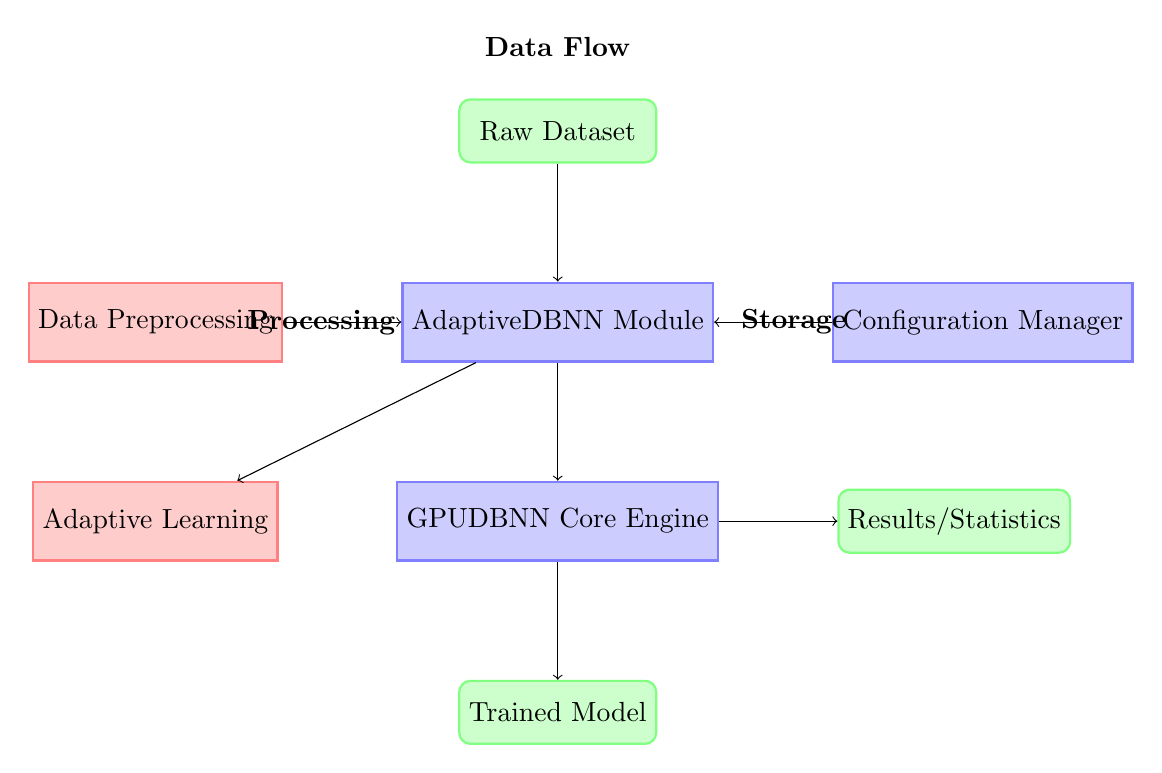
\begin{tikzpicture}[
    node distance=1.5cm,
    module/.style={rectangle, draw=blue!50, fill=blue!20, thick, minimum width=3cm, minimum height=1cm, text centered},
    data/.style={rectangle, draw=green!50, fill=green!20, thick, rounded corners, minimum width=2.5cm, minimum height=0.8cm},
    process/.style={rectangle, draw=red!50, fill=red!20, thick, minimum width=3cm, minimum height=1cm, text centered}
]

% Modules
\node (adaptive) [module] {AdaptiveDBNN Module};
\node (dbnn) [module, below=of adaptive] {GPUDBNN Core Engine};
\node (config) [module, right=of adaptive] {Configuration Manager};

% Data flows
\node (rawdata) [data, above=of adaptive] {Raw Dataset};
\node (results) [data, right=of dbnn] {Results/Statistics};
\node (model) [data, below=of dbnn] {Trained Model};

% Processes
\node (preprocess) [process, left=of adaptive] {Data Preprocessing};
\node (adaptivelearn) [process, below=of preprocess] {Adaptive Learning};

% Connections
\draw[->] (rawdata) -- (adaptive);
\draw[->] (adaptive) -- (dbnn);
\draw[->] (config) -- (adaptive);
\draw[->] (dbnn) -- (results);
\draw[->] (dbnn) -- (model);
\draw[->] (preprocess) -- (adaptive);
\draw[->] (adaptive) -- (adaptivelearn);

% Labels
\node at (0,3.5) {\textbf{Data Flow}};
\node at (-3,0) {\textbf{Processing}};
\node at (3,0) {\textbf{Storage}};

\end{tikzpicture}
\caption{High-level system architecture showing main components and data flows}
\label{fig:architecture}
\end{figure}

\subsection{AdaptiveDBNN Class Structure}

\begin{figure}[h]
\centering
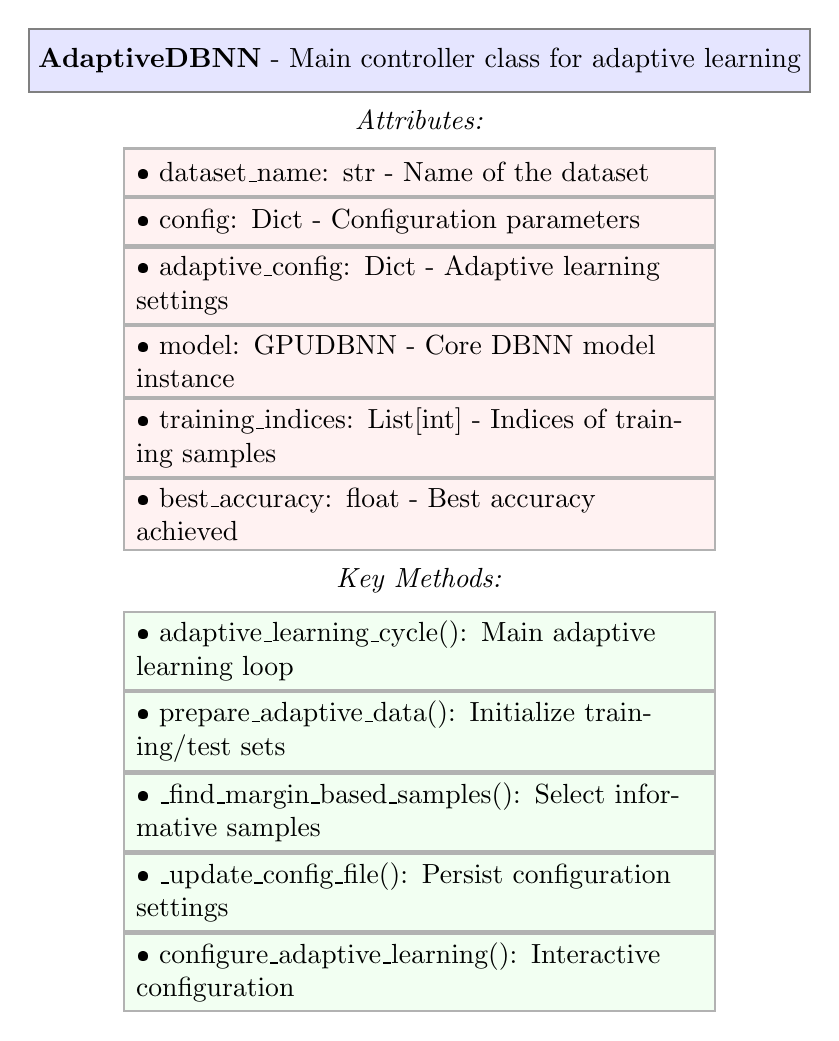
\begin{tikzpicture}[
    class/.style={rectangle, draw=black!50, fill=blue!10, thick, minimum width=8cm, minimum height=0.8cm, text centered},
    method/.style={rectangle, draw=black!30, fill=green!5, thick, minimum width=7.5cm, minimum height=0.6cm, text width=7.2cm, align=left},
    attribute/.style={rectangle, draw=black!30, fill=red!5, thick, minimum width=7.5cm, minimum height=0.6cm, text width=7.2cm, align=left}
]

% Class header
\node (class) [class] {\textbf{AdaptiveDBNN} - Main controller class for adaptive learning};

% Attributes section
\node (attrlabel) [below=0.1cm of class] {\textit{Attributes:}};
\node (attr1) [attribute, below=0.1cm of attrlabel] {• dataset\_name: str - Name of the dataset};
\node (attr2) [attribute, below=0cm of attr1] {• config: Dict - Configuration parameters};
\node (attr3) [attribute, below=0cm of attr2] {• adaptive\_config: Dict - Adaptive learning settings};
\node (attr4) [attribute, below=0cm of attr3] {• model: GPUDBNN - Core DBNN model instance};
\node (attr5) [attribute, below=0cm of attr4] {• training\_indices: List[int] - Indices of training samples};
\node (attr6) [attribute, below=0cm of attr5] {• best\_accuracy: float - Best accuracy achieved};

% Methods section
\node (methodlabel) [below=0.1cm of attr6] {\textit{Key Methods:}};
\node (method1) [method, below=0.1cm of methodlabel] {• adaptive\_learning\_cycle(): Main adaptive learning loop};
\node (method2) [method, below=0cm of method1] {• prepare\_adaptive\_data(): Initialize training/test sets};
\node (method3) [method, below=0cm of method2] {• \_find\_margin\_based\_samples(): Select informative samples};
\node (method4) [method, below=0cm of method3] {• \_update\_config\_file(): Persist configuration settings};
\node (method5) [method, below=0cm of method4] {• configure\_adaptive\_learning(): Interactive configuration};

\end{tikzpicture}
\caption{AdaptiveDBNN class structure with key attributes and methods}
\label{fig:class_structure}
\end{figure}

\section{Mathematical Foundations}

\subsection{Bayesian Framework}

The system implements a Bayesian neural network framework with Gaussian likelihoods:

\[
P(y|x,\theta) = \prod_{i=1}^{N} \mathcal{N}(y_i | f(x_i,\theta), \sigma^2)
\]

Where feature combinations are modeled as multivariate Gaussians:

\[
P(x|y=c) = \frac{1}{(2\pi)^{k/2}|\Sigma_c|^{1/2}} \exp\left(-\frac{1}{2}(x-\mu_c)^T\Sigma_c^{-1}(x-\mu_c)\right)
\]

\subsection{Margin-Based Sample Selection}

The adaptive learning system employs a margin-based approach to select the most informative samples:

\[
\text{margin} = P(y=\hat{y}|x) - P(y=y_{\text{true}}|x)
\]

Where:
\begin{itemize}
\item $P(y=\hat{y}|x)$ is the posterior probability of the predicted class
\item $P(y=y_{\text{true}}|x)$ is the posterior probability of the true class
\end{itemize}

\section{Adaptive Learning Workflow}

\begin{figure}[h]
\centering
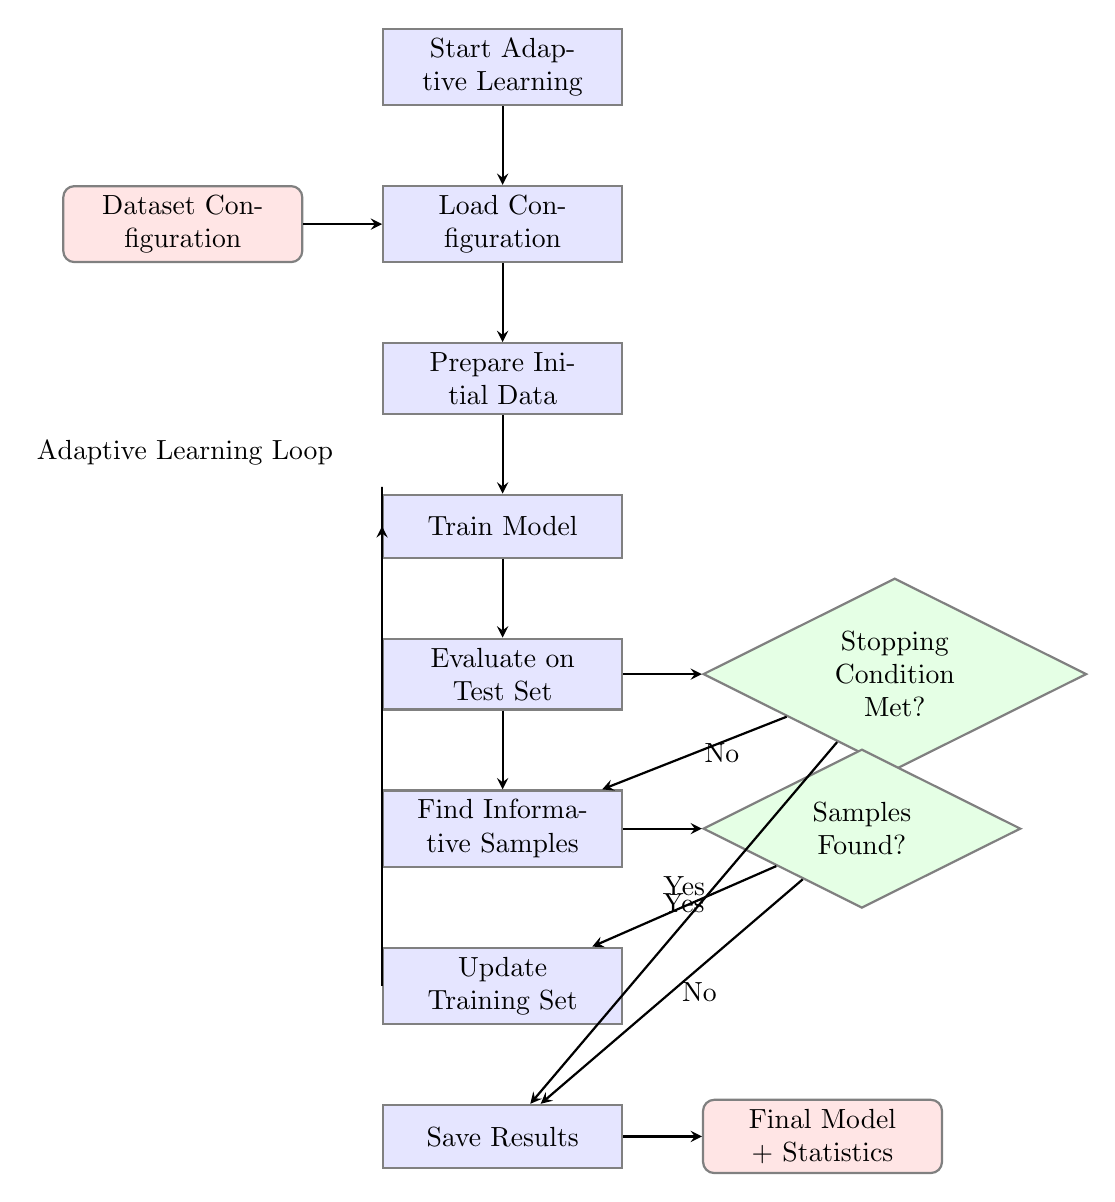
\begin{tikzpicture}[
    process/.style={rectangle, draw=black!50, fill=blue!10, thick, minimum width=3cm, minimum height=0.8cm, text centered, text width=2.8cm},
    decision/.style={diamond, draw=black!50, fill=green!10, thick, aspect=2, text centered, text width=2cm},
    data/.style={rectangle, draw=black!50, fill=red!10, thick, rounded corners, minimum width=3cm, minimum height=0.8cm, text centered, text width=2.8cm},
    arrow/.style={->, >=stealth, thick}
]

% Processes
\node (start) [process] {Start Adaptive Learning};
\node (loadconfig) [process, below=of start] {Load Configuration};
\node (initdata) [process, below=of loadconfig] {Prepare Initial Data};
\node (train) [process, below=of initdata] {Train Model};
\node (evaluate) [process, below=of train] {Evaluate on Test Set};
\node (findsamples) [process, below=of evaluate] {Find Informative Samples};
\node (update) [process, below=of findsamples] {Update Training Set};
\node (save) [process, below=of update] {Save Results};

% Decisions
\node (checkstop) [decision, right=of evaluate] {Stopping Condition Met?};
\node (checksamples) [decision, right=of findsamples] {Samples Found?};

% Data
\node (config) [data, left=of loadconfig] {Dataset Configuration};
\node (results) [data, right=of save] {Final Model + Statistics};

% Connections
\draw[arrow] (start) -- (loadconfig);
\draw[arrow] (loadconfig) -- (initdata);
\draw[arrow] (initdata) -- (train);
\draw[arrow] (train) -- (evaluate);
\draw[arrow] (evaluate) -- (findsamples);
\draw[arrow] (findsamples) -- (checksamples);
\draw[arrow] (checksamples) -- node[above] {Yes} (update);
\draw[arrow] (update) -| ($(initdata.south west)!0.5!(train.south west)$) |- (train.west);
\draw[arrow] (checksamples) -- node[right] {No} (save);
\draw[arrow] (evaluate) -- (checkstop);
\draw[arrow] (checkstop) -- node[above] {Yes} (save);
\draw[arrow] (checkstop) -- node[right] {No} (findsamples);
\draw[arrow] (config) -- (loadconfig);
\draw[arrow] (save) -- (results);

% Loop label
\node at ($(initdata.west)!0.5!(train.west)$) [left=0.5cm] {Adaptive Learning Loop};

\end{tikzpicture}
\caption{Complete adaptive learning workflow}
\label{fig:workflow}
\end{figure}

\section{Configuration System}

\subsection{Configuration File Structure}

The system uses JSON configuration files with the following structure:

\begin{lstlisting}[language=JSON]
{
    "file_path": "dataset.csv",
    "target_column": "target",
    "separator": ",",
    "has_header": true,
    "training_config": {
        "trials": 100,
        "cardinality_threshold": 0.9,
        "learning_rate": 0.1,
        "epochs": 1000,
        "test_fraction": 0.2
    },
    "likelihood_config": {
        "feature_group_size": 2,
        "max_combinations": 1000,
        "update_strategy": 3
    },
    "adaptive_learning": {
        "enable_adaptive": true,
        "initial_samples_per_class": 10,
        "margin": 0.1,
        "max_adaptive_rounds": 15
    },
    "statistics": {
        "enable_confusion_matrix": true,
        "enable_progress_plots": true,
        "save_plots": true
    }
}
\end{lstlisting}

\subsection{Interactive Configuration}

The system provides an interactive configuration interface:

\begin{lstlisting}[language=Python]
def configure_adaptive_learning(self):
    """Interactively configure adaptive learning settings"""
    print("\nConfigure Adaptive Learning Settings")
    print("=" * 50)

    # Get new values from user
    initial_samples = int(input(f"Initial samples per class: ") or 5)
    margin = float(input(f"Margin threshold: ") or 0.1)
    max_rounds = int(input(f"Maximum adaptive rounds: ") or 10)

    # Update settings and config file
    self.adaptive_config.update({
        'initial_samples_per_class': initial_samples,
        'margin': margin,
        'max_adaptive_rounds': max_rounds
    })
    self._update_config_file()
\end{lstlisting}

\section{Algorithms and Implementation}

\subsection{Margin-Based Sample Selection Algorithm}

\begin{algorithm}
\caption{Margin-Based Informative Sample Selection}
\begin{algorithmic}[1]
\Procedure{FindInformativeSamples}{$X, y, predictions, posteriors$}
\State $\text{margin} \gets \text{adaptive\_config}[\text{margin}]$
\State $\text{samples\_to\_add} \gets []$
\State $\text{y\_test} \gets y[\text{test\_indices}]$
\State $\text{failed\_mask} \gets \text{predictions} \neq \text{y\_test}$
\State $\text{failed\_indices} \gets \text{where}(\text{failed\_mask})$

\If{$\text{len}(\text{failed\_indices}) = 0$}
    \State \Return $\text{GetDiverseFallbackSamples}()$
\EndIf

\For{each $\text{idx}$ in $\text{failed\_indices}$}
    \State $\text{true\_class} \gets \text{y\_test}[\text{idx}]$
    \State $\text{pred\_class} \gets \text{predictions}[\text{idx}]$
    \State $\text{margin\_value} \gets \text{posteriors}[\text{idx}, \text{pred\_class}] - \text{posteriors}[\text{idx}, \text{true\_class}]$
    \State $\text{Store margin information}$
\EndFor

\State $\text{max\_margin\_sample} \gets \text{argmax}(\text{margins})$
\State $\text{min\_margin\_sample} \gets \text{argmin}(\text{margins})$
\State $\text{samples\_to\_add} \gets \text{GetMarginBasedSamples}(\text{max\_margin\_sample}, \text{max})$
\State $\text{samples\_to\_add} \gets \text{samples\_to\_add} \cup \text{GetMarginBasedSamples}(\text{min\_margin\_sample}, \text{min})$
\State \Return $\text{samples\_to\_add}$
\EndProcedure
\end{algorithmic}
\end{algorithm}

\section{Technical Specifications}

\subsection{System Requirements}

\begin{itemize}
\item \textbf{Python}: 3.7 or higher
\item \textbf{PyTorch}: GPU/CPU support
\item \textbf{NumPy}: Numerical computations
\item \textbf{Scikit-learn}: Machine learning utilities
\item \textbf{Matplotlib/Seaborn}: Visualization
\item \textbf{Memory}: 8GB minimum, 16GB recommended
\item \textbf{Storage}: Sufficient for datasets and models
\end{itemize}

\subsection{Performance Characteristics}

\begin{itemize}
\item \textbf{Computational Complexity}: $O(n \times f \times c \times e)$
\item \textbf{Memory Usage}: Optimized through pruning and efficient storage
\item \textbf{GPU Acceleration}: Automatic CUDA detection and utilization
\item \textbf{Scalability}: Handles large datasets through streaming
\end{itemize}

\section{Usage Examples}

\subsection{Basic Usage}

\begin{lstlisting}[language=Python]
# Initialize adaptive learning model
adaptive_model = AdaptiveDBNN("my_dataset")

# Configure settings interactively
adaptive_model.configure_adaptive_learning()

# Prepare data and run adaptive learning
X_full, y_full = adaptive_model.prepare_full_data()
best_accuracy, best_indices = adaptive_model.adaptive_learning_cycle(X_full, y_full)
\end{lstlisting}

\subsection{Advanced Configuration}

\begin{lstlisting}[language=Python]
# Manual configuration
config = {
    "adaptive_learning": {
        "initial_samples_per_class": 20,
        "margin": 0.15,
        "max_adaptive_rounds": 20
    },
    "statistics": {
        "enable_confusion_matrix": True,
        "save_plots": True
    }
}

adaptive_model = AdaptiveDBNN("my_dataset", config=config)
\end{lstlisting}

\section{Conclusion}

The Adaptive Deep Bayesian Neural Network framework represents a significant advancement in machine learning systems that can efficiently learn from limited data. The combination of Bayesian methodologies, adaptive learning strategies, and practical implementation considerations makes this framework suitable for a wide range of applications including medical diagnostics, industrial quality control, financial fraud detection, and scientific research.

The system's key strengths include:
\begin{itemize}
\item Intelligent sample selection through margin-based criteria
\item Comprehensive configuration management
\item GPU-accelerated computations
\item Detailed statistical reporting
\item User-friendly interactive interface
\end{itemize}

This documentation provides a comprehensive overview of the system's capabilities, implementation details, and usage patterns. For further information, refer to the source code documentation and example implementations.

\end{document}
